%%
%% Beuth Hochschule für Technik --  Projektarbeit/Projekt-Labor
%%
%% Kapitel 1
%%
%%

\chapter{Introduction}

%Solve babel issue with beuth package: https://texwelt.de/fragen/4775/neuinstallation-texlive-probleme-mit-babel -> sudo apt install texlive-lang-german

TODO convert document to english. for examples Kapitel 1 needs to be Chapter one, so does Inhaltverzeichnis and so 
(4d) (mostly offline)

\section{Python Code within Latex} 
\label{K1_Python in Latex}
%Resource: https://github.com/gpoore/pythontex 
%Run pythontex systems with python3  an no python command: https://github.com/gpoore/pythontex/issues/177
%Configure 	Texstudio to run: 	https://www.alanshawn.com/tech/2019/05/18/scientific-python-5.html (only seems to work for debian package and not for flatpak as it throws the following error: Traceback (most recent call last): File "/app/texlive/bin/x86_64-linux/pythontex", line 55, in <module> import pythontex3 as pythontex ModuleNotFoundError: No module named 'pythontex3' Process exited with error(s) ) The issue is explained here: https://discourse.flathub.org/t/two-questions-about-using-the-texlive-sdk-extension/566 but it is unclear whether Texstudio flatpak packages even uses runtime/org.freedesktop.Sdk.Extension.texlive 	
%https://pypi.org/project/pythontexfigures/ (not necessary, but mabye more confortable for plotting graphs?)
%Plotting with matplotlib: http://conference.scipy.org/proceedings/scipy2012/pdfs/geoffrey_poore.pdf
%Package to install: https://github.com/matplotlib/matplotlib/issues/16911  -> sudo	 apt install cm-super.
%Plot with plotly: https://plotly.com/python/static-image-export/	
%pdflatex -synctex=1 -interaction=nonstopmode %.tex 
%pythontex --interpreter python:python3 (as command )
%even better when you run pythontex --interpreter python:python3 main.tex on console
%http://tug.ctan.org/macros/latex/contrib/pythontex/pythontex_gallery.pdf

\begin{pycode}

print("Python says ``Hello we got it running finally!! YEahjjjjjjo ''")

\end{pycode}

\begin{pyconsole}
x = 400
x = x*2
y = 10
\end{pyconsole}


The variable is $x=\pycon{x}$
The Result of y*2 is $y=\pycon{y}$


\subsection{Integrated matplotlib inline with pythontex}
%If you want to run the code, but don't want to show it, use the \verb+pycode+ environment.
 

\begin{pylabcode}[plotsession]
rc('text', usetex=True)
rc('font', **{'family':'serif', 'serif':['Times']})
rc('font', size=10.0)			
rc('legend', fontsize=10.0)
x = linspace(0, 3*pi)
figure(figsize=(3.25,2))
plot(x, sin(x), label='$\sin(x)$')
plot(x, sin(x)**2, label='$\sin^2(x)$',
linestyle='dashed')
xlabel(r'$x$-axis')
ylabel(r'$y$-axis')
xticks(arange(0, 4*pi, pi), ('$0$',
'$\pi$', '$2\pi$', '$3\pi$'))
axis([0, 3*pi, -1, 1])
legend(loc='lower right')
savefig('myplot.pdf', bbox_inches='tight')
\end{pylabcode}

\begin{figure}[h]
\centering
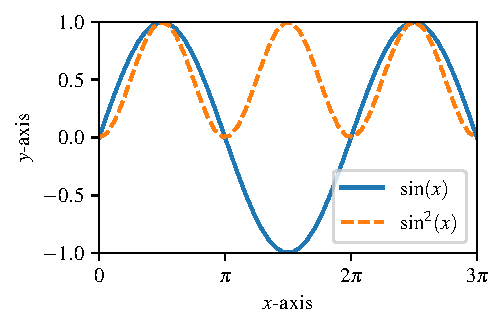
\includegraphics{myplot}
\caption{\label{fig:matplotlib} A plot
created with PythonTeX and Matplotlib}
\end{figure}

\begin{pylabcode}
import plotly.express as px

df = px.data.gapminder().query("continent=='Oceania'")
fig = px.line(df, x="year", y="lifeExp", color='country')
fig.write_image("plotly.pdf")
\end{pylabcode}
	
\begin{figure}[h!]
\centering
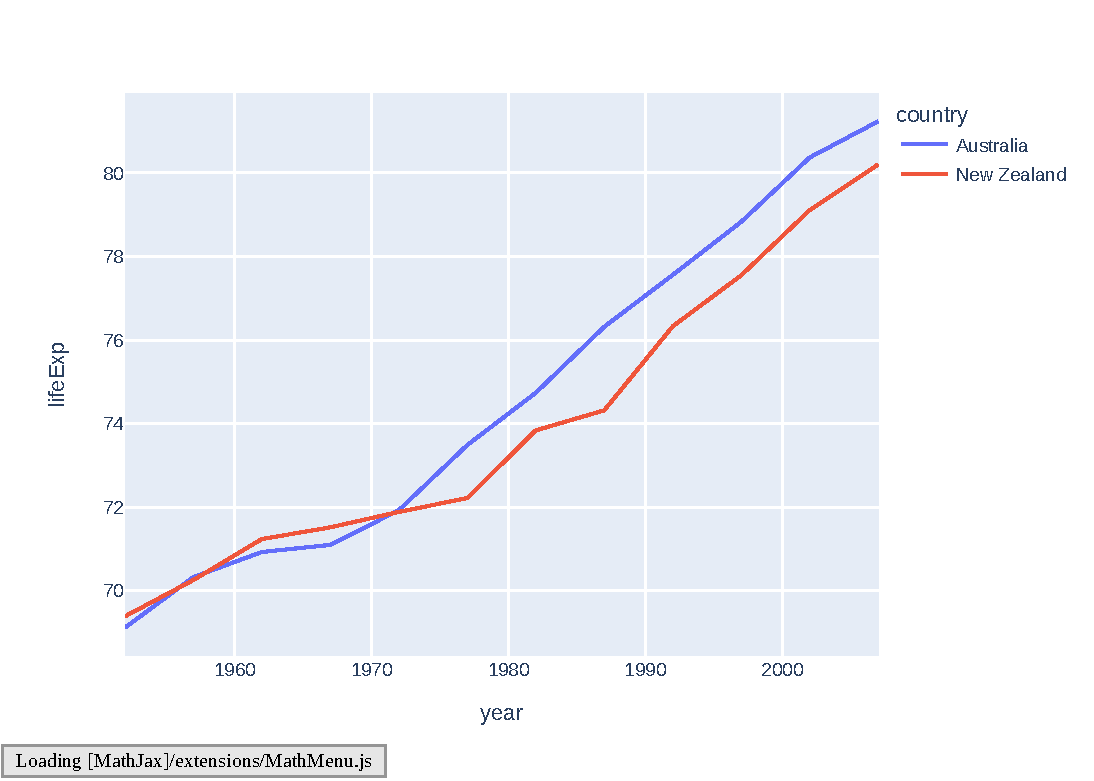
\includegraphics{plotly}
\caption{\label{fig:matplotlib} A plot
created with PythonTeX and Plotly}
\end{figure}

\section{why Kalman, why EKF?}

Other methods are based on auto regressive exogenous (ARX) model or a combination of it and the Kalman Filter.




\chapter{Implementation}



\section{Hardware Setup for validation}

\section{EKF Implementation}
date: (4d)

To design an extended kalman filter algorithm three steps are necessary:
1.The control-input model and the observation model need to be well designed. 
2.The constants inside the models expressed as matrixes need to be definied, which is as well known as parametrisation of the model.  
3.The model needs to be implemented as code running on embedded systems. 

The key to success for a good SoC is a good definition of both models and a good parametrisation. The implementation is independent of the use case and depends on the skills of the programmer, in his  hands lies the optimization of the  code. In case no FPU is available on the micro-controller unit (MCU) fix point arithmetic might be an option.  

Particulary challenging is the parametrization, which is typically done offline \footnote{not done on the microcomtroller unit (MCU) the algorithm is deployed to, thus not on the system running the final algorithm. Offline means on more advanced hardware, which is not available in the final product. See \url{https://en.wikipedia.org/wiki/Online_model} } and required quite advanced equipment. Adaptive extend Kalman Filter is an option where the parameters are determined online, but still AEKF needs to be initialized with parameters not necessary fitting all batteries of a given chemistry (different capacities, different manufacturer). TODO It needs to be researched if it only affects the convergence time or if convergence is not reached at all?  A further advantage of an adaptive filter is that the state of health (SOH) can be determined along the side. 
When simple observation and control-input models are used as in the okra kalman-soc algo, the parametrisation might be much easier? TODO to check if the only parameters OCV(SoC) data can be used generally or only on the batteries they have been measured on. 


Offline parametrizatio: 

Quote: "As a result, many experimental pretests investigating the
effects of the internal and external conditions of a battery on its parameters are required, since the
accuracy of state estimation depends on the quality of the information regarding battery parameter
changes"



"Therefore, some tests data must be available in 
advance to find the parameters of these models."
\cite{hussein2011overview}  \\

 





Gregory Plett says: 
"Two possible approaches: \\


First, an algorithm might somehow adapt the parameter values of the model during operation to match presently observed current–voltage behaviors; but, this \textbf{must be done very carefully to avoid making the model unstable or physically nonmeaningful}. \\

Alternately, a set of models could be pre-computed at different feasible aging points and the model from this set that most closely predicts presently observed current–voltage dynamics could be selected from the set. This second approach guarantees stable and physically meaningful models since all models in the pre-computed set meet these criteria. We propose such an approach here." 
---https://www.sciencedirect.com/science/article/abs/pii/S2352152X18301385?via%3Dihub
In order to have online first algo, the parametrization needs to be done online!. 

As the OCV curve is non-linear the kalman filter can not be used. 

state transition and observation models


\subsection{Definition Mathematics Equations }
 
TODO Make a diagram where you can see the input output and steps\\

%\begin{equation}
%\end{equation}	

Most general form of  state observer equations: \\
$ x_{k+1}=Ax_{k}+Bu_{k} $ (state observer equation) \\
$ y_{k}=Cx_{k}+dDu_{k} $ \ \ \  (output equation)\\ 

$u_{k} \equiv i_{k}$ a control vector (input), defined as the measurement of current through the battery at time $k$. \\ 
$y_{k} \equiv v_{k}$ an observation (or measurement), defined as a voltage measurement of the battery at time $k$. \\
$A = I$  identity matrix f.i $I_{2}=\begin{bmatrix}1&0\\0&1\end{bmatrix}$ \\
$B = \begin{bmatrix}-\frac{\Delta t}{{Q_{C}}}&0\\0&1\end{bmatrix} $  is \textbf{the control-input model}, deduced from  $f({\boldsymbol {x}}_{k},{\boldsymbol {i}}_{k},\Delta t) =  {x}_{k} - \frac{1}{{Q_{C}}}\int_{0}^{\Delta t} {i_{k}\ dk} $ \\
$ C = [0, -R_1, -R_2, ..., M] = H(x_k) $ and $H(x_k) $is the \textbf{observation model} , which maps the state space into the observed space and TODO understand the relationship to $ h(x_k)$ \\ 
$ D = R_0 $ \\


Most general form of Kalman Filter equations: \\

$  {\boldsymbol {x}}_{k+1}=f({\boldsymbol {x}}_{k},{\boldsymbol {u}}_{k})+ {\boldsymbol {w}}_{k} $ \ (State Space equation)  \\
$  {\boldsymbol  {z}}_{{k}}=h({\boldsymbol  {x}}_{{k}})+{\boldsymbol  {v}}_{{k}} $ \ \ \ \ \ \ \ \ \ \ \  \ (Output equation)  \\


$ {\hat  {x}}_{k+1}=\left(A-BK\right){\hat  {x}}_{k}+L\left(y_{k}-{\hat  {y}}_{k}\right) $  ( here $u_{k}$ seems missing)\\

Predicted variables $ \hat{y}_{k}$ and $ \hat{x}_{k} $  are commonly denoted by a "hat" to distinguish them from  $ {y}_{k} $ and $ {x}(k) $  of the physical system. As the state of charge (SoC) denoted as $\hat{x}_{k} = SoC_{k}$  cannot be measured directly it is always a predicted variable, opposed to ${y}(k)$, which is the measured circuit voltage. Consequently $ \hat{y}_{k} = {v}_{k} $ is the predicted circuit voltage also known as measurable output: 

$ {\hat{y}}_{k}=\left(C-DK\right){\hat{x}}_{k} $ 

Input to the extend kalman filter (EKF) is current and voltage measurement and the period of time between these measurements. The initialization of the EKF outputs the initial estimate state of charge  ${x}_{k|k=0} $ another input to the EKF. 

{System's dynamic model} \\
The $f() $ function is defined as the $ f({\boldsymbol {x}}_{k},{\boldsymbol {i}}_{k},\Delta{t}) = {x}_{k} - \frac{1}{{Q_{C}}}\int_{0}^{\Delta t} {i_{k}\ dk} $ or more discrete $f({x}_{k},{i}_{k},\Delta{t}) = {x}_{k} - \frac{\Delta t}{Q_{C}} i_{k} $, thus current measurement $ {i}_{k} $ 
The $h({\boldsymbol {x}}_{{k}})$ function is defined as the OCV lookup table. A general OCV lookup table for the battery chemistry can be used or for better results a specific OCV lookup established by offline measurements for  the given battery should be used. 
To further improve the OCV prediction a correction of it can be performed by a equivalent circuit model (ECM) of the battery feeded by the current measurement used to predict the SoC: 
$ {v}_{k} = {D} \ {OCV}({z}_{k}) + C {x}_{k}  +  D {i}_{k}  $ 
with $ C = [0, -R_1, -R_2, ..., M] $ and $ D = R_0 $

-Measurement equation, input (measured voltage, OCV lookup table, current if the correction with a Enhanced Self-Correcting (ESC) Cell Model /ECM) -> output SOC)
equation should be use standard letters: filterpy, wikipedia, gregoryPlett, Step by Step Guide

After having defined the observation and control-input model as matrices and described their meaning in case of SoC estimation we proceed to the functioning of the EKF, which is typically divided into to steps, Predict and Update. 

In the \textbf{predict} step a future state of charge estimate  $\hat x_{k+1}$ is predicted based on the current state of charge estimate $\hat x_k$ and the current $i_k$ during the period $\Delta t$ (between $k$ and $k+1$) by calculating $ \mathbf{\hat x_{k+1}=Ax_{k}+Bu_{k}} $ Moreover an estimate of the covariance $P_{k+1}x$ is calculated based on noise covariances $Q_k$ and current $P_k$ (wiki: a measure of the estimated uncertainty of the prediction of the system's state)  $\mathbf {P} _{k+1}=\mathbf {B} _{k}\mathbf {P} _{k}\mathbf {B} _{k}^{\textsf {T}}+\mathbf {Q} _{k} $

In the \textbf{update} step  \\
$ \mathbf {K} _{k}=\mathbf {P} _{k+1}\mathbf {H} _{k}^ \textsf {T} (  \mathbf \mathbf {H} _{k}\mathbf {P} _{k+1}\mathbf {H} _{k}^{\textsf {T}+\mathbf {R} _{k})^{-1}}$  is the kalman gain, which weights whether the SoC based on the measurement of the circuit voltage $v_k$ is more trusted than the SoC prediction based on current $i_k$ \\
$ {\hat {\mathbf {x} }}_{k}=(\mathbf {I} -\mathbf {K} _{k}\mathbf {H} _{k})({\hat {\mathbf {x} }}_{k+1})+(\mathbf {K} _{k})(\mathbf {H} _{k}\mathbf {\hat x} _{k}+\mathbf {v} _{k}) $ TODO update $\hat x_k$ because one can not now want one want to calculate\\  

$ \mathbf {P} _{k+1}=\left(\mathbf {I} -\mathbf {K} _{k+1}\mathbf {H} _{k+1}\right)\mathbf {P} _{k} $ update of the covariance TODO is $H_{k}$ the same as OCV? \\

$\mathbf{R_k}$ the covariance of the observation noise  \\

Most general equation of extended kalman filter EKF: \\

$ \mathbf {x}_{k}=f(\mathbf {x} _{k-1},\mathbf {u}_{k})+\mathbf {w}_{k}\ $ (state transition model) \\
$\mathbf {z}_{k}=h(\mathbf {x} _{k})+\mathbf {v}_{k}$ \ \ \ \ \ \ \ \ \ \ \  \ (observation model)  \\
\emph{f} ->  predicted state from the previous estimate  \\
\emph{h} ->  compute the predicted measurement from the predicted state \\


\textbf{Predict} \\
${\displaystyle {\hat {\boldsymbol {x}}}_{k|k-1}=f({\hat {\boldsymbol {x}}}_{k-1|k-1},{\boldsymbol {u}}_{k})} $ \\
${\displaystyle {\boldsymbol {P}}_{k|k-1}={{\boldsymbol {F}}_{k}}{\boldsymbol {P}}_{k-1|k-1}{{\boldsymbol {F}}_{k}^{\top }}+{\boldsymbol {Q}}_{k}}$ \\

\textbf{Update} \\
${\tilde  {{\boldsymbol  {y}}}}_{{k}}={\boldsymbol  {z}}_{{k}}-h({\hat  {{\boldsymbol  {x}}}}_{{k|k-1}})$ \\
${\boldsymbol  {S}}_{{k}}={{{\boldsymbol  {H}}_{{k}}}}{\boldsymbol  {P}}_{{k|k-1}}{{{\boldsymbol  {H}}_{{k}}^{\top }}}+{\boldsymbol  {R}}_{{k}}$ \\
${\boldsymbol  {K}}_{{k}}={\boldsymbol  {P}}_{{k|k-1}}{{{\boldsymbol  {H}}_{{k}}^{\top }}}{\boldsymbol  {S}}_{{k}}^{{-1}}$ \\
${\hat  {{\boldsymbol  {x}}}}_{{k|k}}={\hat  {{\boldsymbol  {x}}}}_{{k|k-1}}+{\boldsymbol  {K}}_{{k}}{\tilde  {{\boldsymbol  {y}}}}_{{k}}$ \\
${\boldsymbol  {P}}_{{k|k}}=({\boldsymbol  {I}}-{\boldsymbol  {K}}_{{k}}{{{\boldsymbol  {H}}_{{k}}}}){\boldsymbol  {P}}_{{k|k-1}}$ \\




\section{Kalman-SoC}
A Fork of Okra-Solar Algorithm. \

Features: \

-Works without the input of a Equivalent Circuit Model (ECM) specific to the physical battery, which would need to be parameterized doing advanced measurements during charging and discharging of the battery. 

-Inputs: Current and Voltage Measurements and OCV Lookup Table

-Outputs: SoC in \%Wh

TODO Discuss the Code Snippets? But Some Code in Appendix or reference Github Repo only? 
\chapter{Validation}


\ref{K1_Python in Latex} has all the info how to integrate graphs here. 
 
Discuss results.  (4d)

\chapter{Outlook}

Promising articles and/or methods for online parameter estimation: \\ 

\textbf{online parameter estimation} from the ARX model  \cite{tran2017state}

\cite{xia2018online}
\cite{wang2021augmented}